
\chapter{O Processo}

O conceito de processo normalmente está relacionado ao programa em
execução, ou seja, ao conjunto de instruções a ser processado. Porém,
outros elementos são necessário para a correta execução das
instruções, tais como, arquivos abertos, estado do processador, número
de \thread{}s, variáveis acessíveis e mapeamento de memória. O
gerenciamento do processo envolve a coordenação de todos os detalhes
relacionados a estes elementos.

\section{Estados de um processo}

A Figura~\ref{fig:proc:states} mostra o diagrama de estados de um
processo, que pode estar em um dos seguintes estados:

\begin{center}
  {\tt\{PRONTO, EXECUTANDO, ESPERANDO, MORTO\}.}
\end{center}

\begin{description}
\item[\tt PRONTO] O processo encontra na fila de processos que podem
  ser executados. Neste estado, o processo pode ter acabado de passar
  pelo processo de criação, ter sido retirado da execução ou ter
  recebido um sinal para passar do estado {\tt ESPERANDO} para o
  estado {\tt PRONTO}, normalmente ao término de atendimento de uma
  requisição de E/S.
\item[\tt EXECUTANDO] O processo está em execução no processador.
\item[\tt ESPERANDO] O processo está ``adormecido'', aguardando a
  alguma condição ser satisfeita, como um interrupção de hardware, uma
  liberação de recursos ou o recebimento de um sinal. Havendo a
  satisfação da condição, o processo passa para o estado {\tt PRONTO}.
\item[\tt MORTO] O processo terminou a sua execução.
\end{description}

\begin{figure}[ht]
  \centering
  \input \imgdir/states
  \caption{Estados de um processo.}
  \label{fig:proc:states}
\end{figure}

Durante a criação do processo uma estrutura chamada PCB
(\textit{Process Block Control}) ou bloco de controle do processo é
gerada para armazenar informações utilizadas pelo sistema operacional
no gerenciamento do processo. A Figura~\ref{proc:fig:pcb} ilustra
alguns atributos normalmente armazenados no PCB para controle do
processo. 

Logo que um processo é criado, recebe um identificador PID
(\textit{Process IDentification}), normalmente um número inteiro, para
diferenciá-lo dos demais processos. No PCB também é
armazernado os seguintes atributos, dentre outros:

\begin{itemize}
\item O {\bf estado} em que o processo se encontra;
\item O {\bf contador de programa}, ou seja, qual a próxima instrução a ser
  executada,
\item O mapeamento entre as variáveis do programa e os {\bf registradores}
  do processador;
\item {\bf Limites de memória} que o programa pode utilizar;
\item {\bf Lista de arquivos abertos} utilizados pelos processo.
\end{itemize}

\def\recbase{5}
\def\recheight{1}

\begin{figure}

\begin{center}
  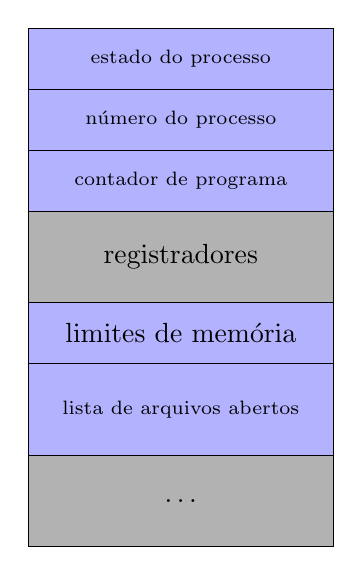
\begin{tikzpicture}[every rectangle/.style={minimum width=\recbase},
    scale=0.775,mem/.style={fill=gray!60},
    var/.style={fill=blue!30}]
    
    \draw[var] (0,2+5.5*\recheight) rectangle (\recbase,2+6.5*\recheight)
    node[midway] {\scriptsize{estado do processo}};
    \draw[var] (0,2+4.5*\recheight) rectangle (\recbase,2+5.5*\recheight)
    node[midway] {\scriptsize{número do processo}};
    \draw[var] (0,2+3.5*\recheight) rectangle (\recbase,2+4.5*\recheight)
    node[midway] {\scriptsize{contador de programa}};
    \draw[mem] (0,2+2*\recheight) rectangle (\recbase,2+3.5*\recheight) node[midway] {registradores};
    \draw[var] (0,2+\recheight) rectangle (\recbase,2+2*\recheight) node[midway] {limites de
    memória};
    \draw[var] (0,1.5) rectangle (\recbase,2+\recheight) node[midway] {\scriptsize{lista de
    arquivos abertos}};
    \draw[mem] (0,0) rectangle (\recbase,1.5*\recheight) node[midway] {$\ldots$};
  \end{tikzpicture}
\end{center}

\caption{Bloco de controle do processo.}
\label{proc:fig:pcb}

\end{figure}


No sistema operacional GNU/Linux os atributos de um processo são
armazenados em uma variável do tipo {\tt struct} conforme mostrado na
Figura~\ref{proc:src:sched}.

\begin{figure}[ht]
\lstinputlisting[frame=single,firstline=13]{../sched/sched.h}
\label{proc:src:sched}
\caption{Listagem da estrutura de dados do PCB do GNU/Linux.}
\end{figure}

O estado do processo é armazenado na variável {\tt state}, a
indetificação na variável {\tt pid}, o usuário ao qual o processo
pertence na variável {\tt loginuid}. O restante das variáveis são
utilizadas para controle do estado do processo, ou seja, para fins de
escalonamento que será visto na seção~\ref{sec:sched}.